%sse
\documentclass[../../main/main.tex]{subfiles}


\begin{document}
\title{Systems Security Engineering}


%%%%%%%%%%%%%%%%%%%%% Chapter CSBD ACL %%%%%%%%%%%%%%%
\chapter{Systems Security Engineering \& Patrol Base Operations}\label{chp:sse}


       %%%%%%%%%%%%%%%%%% Section Systems %%%%%%%%%%%%%%%%
\section{The Systems Perspective}\label{sec:systems}
A system is a set of interacting and interdependent components that act as a whole to perform some behavior or function.  Examples of systems include the human body, socio-political systems, and computer systems. 

The patrol base operations satisfy this definition of a system.  As a whole, the patrol base operations perform some function(s).  This function is described in the Ranger Handbook \cite{rangermanual} and discussed in section \ref{sec:pb}.  The patrol base operations are comprised of interdependent and interacting components.  In general these components are the individual soldiers.  But, the way this master thesis defines the patrol base operations, the definition of a component varies.

This master thesis defines the patrol base operations as a system of systems.  More specifically, this thesis models the patrol base operations as a hierarchy of \glsentrylongpl{ssm}.  Chapter \ref{chp:ssmmodel} describes \glsentryshortpl{ssm} in general.   Section \ref{sec:modelingpb} describes this model of the patrol base operations.  

This model presents the patrol base operations as a hierarchy wherein each level of the hierarchy represents a decreasing level of abstraction.  At the top and most abstract level, the components are phases of the patrol base operations.  These phases commence in a sequential order to achieve the goal of the patrol base operations.  Each lower level of the hierarchy is composed of less abstract phases. At each level, the components function sequentially (typically) to achieve the ultimate goal.  

This system of systems also contains non-hierarchically defined components.  For example, an escape-level component models situations wherein the patrol base operations are aborted.  The escape level component is reachable from any component at any level of the hierarchy.  Soldiers also function within this system of systems in a non-hierarchical manner.  However, CSBD was not applied to the soldier module for this master thesis.  Nevertheless, they were discussed in detail and are discussed in the Discussions chapter \ref{chp:discussion} of this thesis.

In this way, the patrol base operations represent a system and are amiable to the systems engineering perspective.  

     %%%%%%%%%%%%%%%%%% Section Systems Engineering %%%%%%%%%%
\section{Systems Engineering}\label{sec:se}
The recognized authoritative standard on systems engineering is ISO/IEC/IEEE 15288 \cite{iso15288}.  This document is titled "Systems And Software Engineering--System Life Cycle Processing."  A precursor to this standard is ISO/IEC TR 24748 1 \cite{iso24748} titled "Systems And Software Engineering--Life Cycle Management--Part 1: Guide for Life Cycle Management."   These are the primary sources for this section.

Systems engineering is an interdisciplinary approach aimed at solving problems involved in the various phases of the life cycle of a system.  ISO/IEC/IEEE 15288 and ISO/IEC TR 24748 1 define five major phases of the this life cycle: concept, development, production, utilization, support, and retirement.
  
This master thesis focuses on the \glsentrylong{csbd} (\glsentryshort{csbd}).  The key premise of \glsentryshort{csbd} is that security should be built into the systems from the start, i.e., the design phase.  This is the leading notion in systems engineering and its sub-discipline \glsentrylong {sse}.  

  The aim is to model the patrol base operations in a manner that is amiable to verifying specific security properties of the system.  Specifically, the patrol base operations must satisfy the property of complete mediation. 


But, this thesis does not aim to build a new system.  Rather this thesis remodels an existing system.   This is necessary because the goal of this thesis is to determine whether or not it is possible to verify the specific security properties on the subclass of systems that we are exploring.  Most people would agree that testing a new method on a new system would be unwise.  This is why this thesis did not do that.    


This approach has the side-effect of also demonstrating CSBDs utility in the life-cycle phase of systems engineering.  It follows readily from the news today that many systems are not designed with security in mind.  Eliminating already-in-use systems and legacy systems may not always be practical or desirable.  Nevertheless, security remains an important aspect of system performance.  This, in part, justifies a re-look at (or remodeling of)  of an already existing system.


There are additional benefits to systematically modeling the patrol base operations in a way that is amiable to formal verification.  This type of thinking provides new insights and suggests areas for improvement\footnote{The subject matter expert who focused on the details of the patrol base operations also noted areas for improvement.  He was not available to provide details at the writing of this master thesis.}.  This is a known benefit.  For example, Wikipedia \cite{wikiformalmethods} notes that "Sometimes, the motivation for proving the correctness of a system is not the obvious need for reassurance of the correctness of the system, but a desire to understand the system better."  A greater understanding of a system applies to all phases of systems engineering.

     %%%%%%%%%%%%%%%%%% NIST %%%%%%%%%%%%%%%%%%%%%
\section{NIST Special Publication 800-160}
One work in the field of \glsentrylong{sse} is such a critical component to the field of \glsentryshort{sse} that it warrants pointing out. The \glsentrylong{nist} (NIST) defines its mission as such: "To promote U.S. innovation and industrial competitiveness by advancing measurement science, standards, and technology in ways that enhance economic security and improve our quality of life." \cite{nistmission}.  As their name suggests, NIST develops standards for various industries of relevance to the nation.   

The relevant standard for \glsentryshort{sse} is NIST Special Publication 800-160 Volumes 1 and 2. The title of volume 1 is "Systems Security Engineering
Considerations for a Multidisciplinary Approach in the Engineering of Trustworthy Secure Systems."  The title of volume 2 is "Systems Security Engineering Cyber Resiliency Considerations for the Engineering of Trustworthy Secure Systems."   These, in particular volume 1, are the primary sources for the following two sections.  

     %%%%%%%%%%%%%%%%%% Section Systems Security Engineering %%%%%%
\section{Systems Security Engineering}\label{sec:sse} 
Systems security engineering (\glsentryshort{sse}) is a sub-discipline of systems engineering.  Figure \ref{fig:nist800160} shows \glsentryshort{sse} in relation to systems engineering and other sub-disciplines of \glsentryshort{sse}.  This master thesis falls into one of the Security Specialties in this diagram.

\begin{figure}[h]
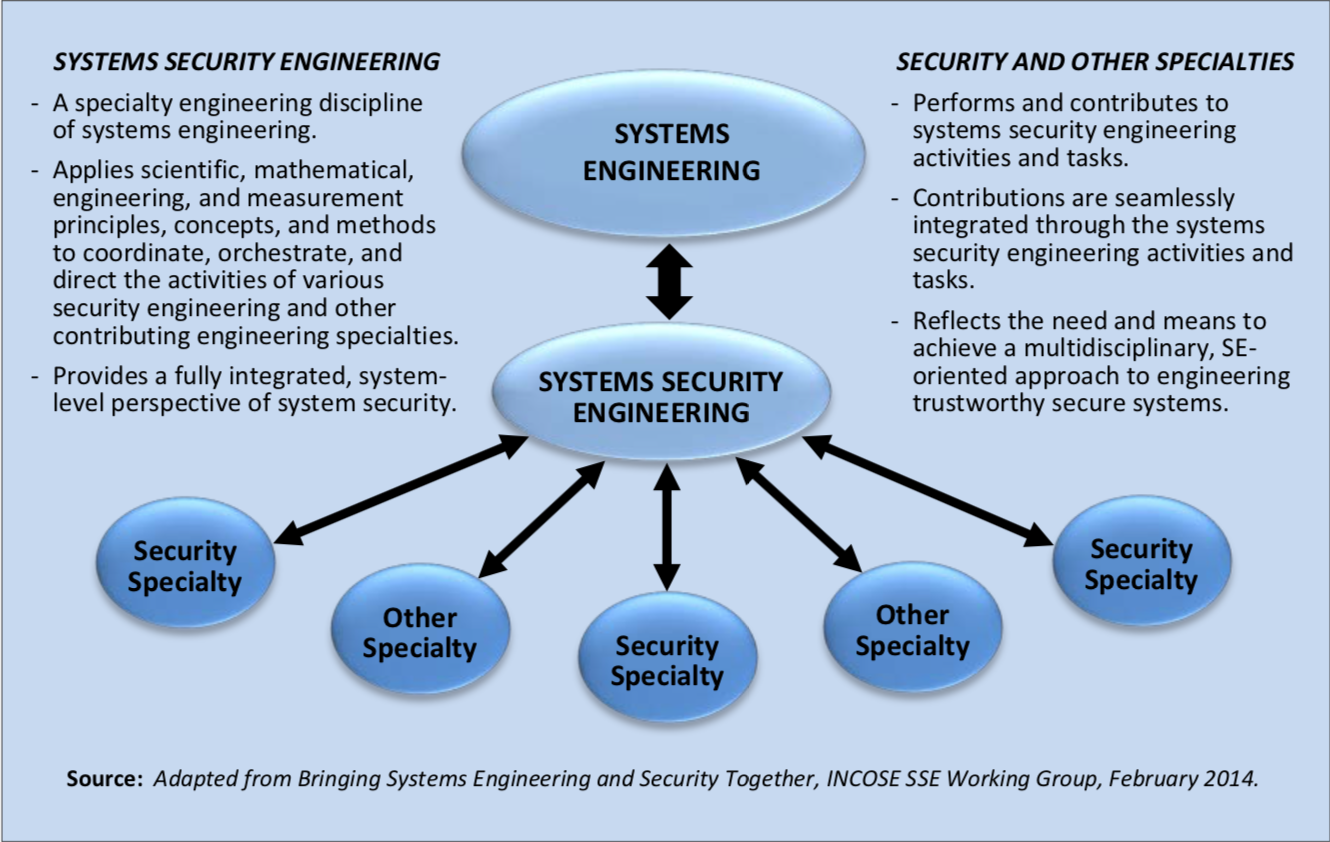
\includegraphics[width=\linewidth]{../figures/seincontext.png}
\caption{\label{fig:nist800160}Systems security engineering in relation to systems engineering. (Image from \glsentryshort{nist} Special Publication 800-160: Systems Security Engineering Considerations for a Multidisciplinary Approach in the Engineering of Trustworthy Secure Systems.)}
\end{figure}

According to \glsentryshort{nist} Special Publication 800-160, "Systems security engineering focuses on the protection of stakeholder and system assets so as to exercise control over asset loss and the associated consequences."  Three key concepts in \glsentryshort{sse} are stakeholder, asset, and unacceptable losses.  In modeling the patrol base operations, this thesis first defines these key concepts.  

\begin{description}
\item[ Stakeholder]  The stakeholder controls the design of the system.  The stakeholder defines what the system should do.  The stakeholder also defines what the system should not do and what are unacceptable losses.  The stakeholder for the patrol base operations are ultimately the U.S. military.  This was critical to the original design of the patrol base operations.  But, this thesis has a different purpose, that of demonstrating specific security properties of the patrol base operations using CSBD.  These security properties are that of complete mediation.  For this master thesis, the stakeholders are everyone involved in this research.  
\item[Asset] An asset is anything that is of value to the stakeholder.   In the patrol base operations, this includes soldiers, equipment, and the mission.
\item[Unacceptable losses] Unacceptable losses are self-defining.  Unacceptable losses for the patrol base operations are defined broadly as any event that would cause the patrol base operation as a whole to abort.  These are: contact with the enemy, casualties, a change in mission from higher-up.
\end{description}

It is also a critical objective of \glsentryshort{sse} to identify and define the security goals of the stakeholder in a way that minimizes asset loss and avoids unacceptable losses.  The security properties of the patrol base operations are already built-in to the design of the operations from the Ranger Handbook.  These are undoubtedly the result of years of military expertise.  Our goal is not to define the security features of the patrol base operations, but to describe them in manner amiable to verification of complete mediation.  Identification of assets and unacceptable losses from the Ranger Handbook is sufficient to do this.

To cover the unacceptable losses, this master thesis models an escape-level \glsentrylong{ssm} (SSM).  If at any phase in the patrol base operations any authenticated principal (i.e., the platoon leader) reports an abortable event, the escape-level \glsentryshort{ssm} will abort the patrol base operations. This includes casualties or unacceptable equipment failure.  By creating one escape-level \glsentryshort{ssm}, this thesis creates an modularized yet expandable treatement of unacceptable losses.


To further describe the model of the patrol base operations in the context of \glsentryshort{sse}, a few more concepts are necessary.  

\section{Systems Security Engineering Framework}\label{sssec:sseframework}
NIST 800-160 describes the systems security engineering framework shown in figure \ref{sseframework} as "contexts within which systems security engineering activities are conducted."  CSBD focuses primarily on demonstrating trustworthiness.  Nevertheless, this master thesis also addressed other aspects of the framework.  

\begin{figure}[h]
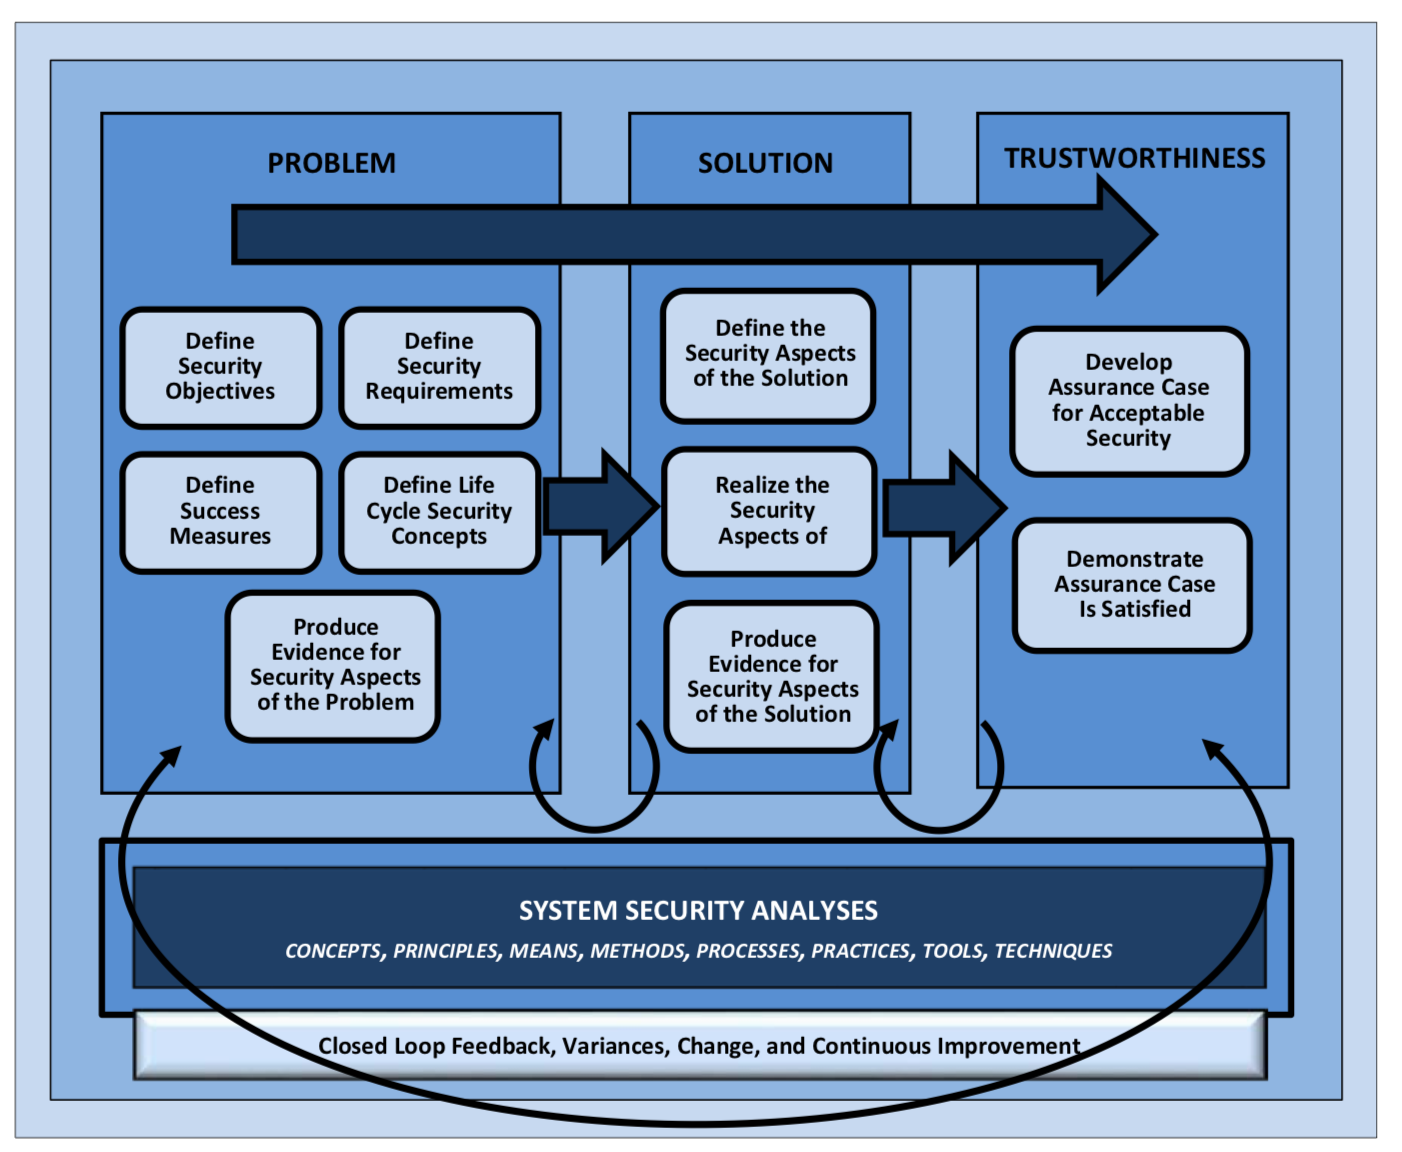
\includegraphics[width=\linewidth]{../figures/sseframework}
\caption{\label{sseframework}Systems security engineering Framework. (Image from \glsentryshort{nist} Special Publication 800-160: Systems Security Engineering Considerations for a Multidisciplinary Approach in the Engineering of Trustworthy Secure Systems.)}
\end{figure}

The problem and solution phases for the patrol base operations take a different approach in the context of this master thesis. It is not our goal to outline the potential security threats and then to find solutions for them.  This was, hopefully, already done when the patrol base operations were originally defined.  Nonetheless, it is necessary to identify the problem and solution within the patrol base operations in order to verify their security properties.  


\subsection{Problem}
The security objective from the perspective of this master thesis is to ensure complete mediation of all actions.  Complete mediation requires that we identify objects to be accessed, the accessors, the means of authenticating the accessors, and the a policy for authentication.  

The objects to be accessed varies at each level of abstraction. At the top and most abstract level, the objects are the transitions.  That is, control over the transitions between phases (or states) of the patrol base operations are to be protected.  Objects are defined similarly for each module and at each level for the entire hierarchy of the model.  These are deducible from the descriptions of each module (or \glsentryshort{ssm}) in their appropriate section (see section \ref{ssec:omnilevel} to start).  For the sake of brevity, this section only discusses the top level to illustrate the key concepts.  

The accessors are the leaders designated at each level of abstraction.  The best way to negotiate access to objects is by the principle of least privilege.  This principle assigns privilege to only those who are deemed necessary and to no others.  At the top level, the platoon leader (and only the platoon leader) is designated as the accessor. This means that only the platoon leader can issue commands to move-on to the next phase (or state) in the patrol base operations. Some of the other modules have more than one accessor.  These accessors are typically assigned privileges to specific objects within the module.  The rights of each accessor are determined by the policy.

In the real patrol base operations, soldiers recognize each other by face.  Thus, it is sufficient to just authenticate the platoon leader at each level without requiring any passwords or other means of authentication\footnote{The author and subject matter expert discussed authentication in the context of an accountability system wherein passwords or chips were required for authentication.  But, we did not implement such authentication techniques in this project.}.

Policy is determined for each module and at each level of the patrol base operations model.  The model includes not only "who" is authorized to do what, but also what preconditions are necessary prior to authorization.  This is more complicated than authentication.

At the top level, there are only two requirements for the patrol base operations to move to the next phase of the operations: (1) the previous phase is complete, and (2) the platoon leader issues the command to move to the next phase.  This creates a potential conflict between the goal of modularizing each component and creating a hierarchy wherein each level of the hierarchy expands upon the one above it.  In general, If the top level requires some signal from the lower level that it is complete, then these two levels are not independent. 

To solve this problem, an OMNI level module is created.  The OMNI level module is thought of as all-knowing.  This module relays information from all modules as needed.  With this construct, the top level does not need to "know" if the lower level module is complete.  It only needs to know that the OMNI level says that it is complete.  The OMNI level is given the authority to determine when any module is complete.

With this solution in mind, the top level policy looks like this.


\fbox{
\parbox{\linewidth}{
\begin{center}
\textit{if OMNI-Level says the previous phase is complete\footnote{For those who have read ahead, the reader may recognize that this does not follow logically from the inference rules.  The actual implementation of this policy requires the two inputs on the first and second line and returns that output on the final line.  Within the policy is the requirement that OMNI Level has the authority to determine that the previous phase is complete.  To state this in the text here would only clutter it and confuse the reader.}, and \\
Platoon Leader says move to the next phase\\
 then Platoon Leader has the authority to move to the next phase}
\end{center}
}}

\subsection{Solution}
The simplest solution to this problem is to model the patrol base operations as a hierarchy of secure state machines (\glsentryshort{ssm}).  The hierarchy simplifies the design of the solution by creating decreasing levels of abstraction with multiple modules at each level.  This allows for focus on one level and one module at time. This essentially amounts to a system of systems approach.  Furthermore, this allows for greater separation of work.  After one level of the hierarchy is complete, CSBD is applied to that level while the next level of the hierarchy is being designed.

\glsentryshortpl{ssm} are readily defined with complete mediation embedded into their design.  \glsentryshortpl{ssm} are discussed in detail in Chapter \ref{chp:ssmmodel}.  In fact, a parameterizable model of an \glsentryshort{ssm}\footnote{This SSM was modeled and implemented in HOL by Professor Shiu-kai Chin and used with his permission.} was already designed and implemented in HOL prior to the start of this project.  The constraints of this project suggested Improvements\footnote{Because these improvements were significant, the original author (Professor Shiu-kai Chin) made them.} to this parameterizable \glsentryshort{ssm}\footnote{Much to the chagrin of the author, a significant portion of the SSMs had to be redone with the new parameterizable SSM.}.

The most useful property of the \glsentryshort{ssm} is that complete mediation is made a condition for transitions among states.  That is, to transition from one state to another the accessor (requestor) must be properly authenticated and authorized. Authentication and authorization are described above in the description of the problem.   For example, at the top level, transition commands in an \glsentryshort{ssm} look like this.

\fbox{
\parbox{\linewidth}{
\begin{center}
\textit{if Platoon Leader's identity is authenticated, and\\
         Platoon Leader says move to the next phase, and \\
         Platoon Leader has the authority to move to the next phase\\
         then move to the next phase.}
\end{center}
}}

The first line ensures authentication of the Platoon Leader.  The second line is a request from the Platoon Leader to access the object (i.e., move to the next phase).  The third line is the output of a policy as described in the section above and shown in the box above. 

Note that this is an "if and only if" conditional.  This means that if the Platoon Leader is authenticated, authorized on, and issues the command then the command is executed.  It also means the converse.  If the command is executed, then the Platoon Leader is authenticated, authorized on, and issues the command to do so.  

\subsection{Trustworthiness}


There are two requirement for trustworthiness relevant to this master thesis: (1) Defining trustworthiness for the purposes of this master thesis, and (2) demonstrating that trustworthiness is achieved.  The former is easy for this model.  This master thesis focuses on the trustworthiness aspect of \glsentryshort{sse}.  Therefore, this master thesis elaborates on trustworthiness in the following sections.

\section{Trustworthiness}\label{sssec:trustworthiness}
This master thesis defines trustworthiness in the context of complete mediation\footnote{Note that there are certainly other measures of trustworthiness in any system.  Nonetheless, the focus of this thesis is to demonstrate CSBD as a viable method for one aspect of the systems security engineering process.  The author does not aim to claim that the patrol base operations are deemed trustworthy solely because they satisfy the property of complete mediation.  CSBD is one piece of the larger puzzle.}.  Therefore, a measure of trustworthiness is weather or not the patrol base operations satisfy the properties of complete mediation.  There are two aspects to this: (1) building complete mediation into the model of the patrol base operations, and (2) demonstrating that this is indeed the fact.  

\subsection{Verification \& Documentation}\label{sssec:sseframework}

\subsubsection{Verification}
\subsubsection{Formal Verification}

\subsubsection{Documentation}


A common idiom of science and engineering is "if you didn't document it then it didn't happen."  There is some leeway in engineering because the presence of a system is indicative that "you did it." However, this hides the important details regarding the security of the system.  Maybe "you did it" but "did you do it right?"  This is where documentation is important. 

'''systems security engineering provides a sufficient base of evidence that supports claims that the desired level of trustworthiness has been achieved..."


\subsection{Reproducibility}\label{ssec:reproducibility}
\subsection{Accountability}\label{ssec:accountability}
Internet Hall of Fame Inductee Vint Cerf commented on the importance of accountability in \glsentryshort{sse} at a recorded conference in 2016.  The conference titled "Exploring the Dimensions of Trustworthiness: Challenges and Opportunities" was presented by NIST.  

\subsection{Assurance Claims}\label{ssec:assurance}



\end{document}